\documentclass{beamer}
\mode<presentation>
{
    \usetheme{Warsaw}      % or try Darmstadt, Madrid, Warsaw, ...
    \usecolortheme{beaver} % or try albatross, beaver, crane, ...
    \usefonttheme{default}  % or try serif, structurebold, ...
    \setbeamertemplate{navigation symbols}{}
    \setbeamertemplate{caption}[numbered]
    \setbeamertemplate{footline}[frame number]
}

\usepackage[english]{babel}
\usepackage[utf8]{inputenc}
\usepackage{pgfpages}
\usepackage{color}
\usepackage{listings}

\definecolor{grey}{rgb}{0.9,0.9,0.9}

\newcommand{\dbf}[1]{\operatorname{dbf}(#1)}

\title {Using DIT in the DBF feasibility test}
\author {Thomas Chapeaux}
\institute {ECE Paris}
\date {July 2013}

\begin{document}

\begin{frame}
    \titlepage
\end{frame}

\begin{frame}{Outline}
    \tableofcontents
\end{frame}

\section{Demand Bound Function (DBF)}

\begin{frame}{Outline}
    \tableofcontents[currentsection]
\end{frame}

\subsection{Definition}

\begin{frame}{Definition}
    \begin{definition}
    The \textbf{demand-bound function (DBF)}, defined for a task set $\tau$ and noted $\dbf{t}$, is equal to the maximal cumulated execution time of jobs of $\tau$ contained in any interval of length $t$.
    \end{definition}

    In the synchronous case, a closed form expression is $$\dbf{t} = \sum_{i=1}^{n} \operatorname{max} \{ 0, \lfloor \frac{t - D_i}{T_i} \rfloor + 1 \} \, C_i$$
\end{frame}

\subsection{Feasibility test}

\begin{frame}{Feasibility test}
    \begin{theorem}
        $$\text{$(\tau_1, ..., \tau_n)$ is feasible} \iff \dbf{t} \leq t \; \forall t$$
    \end{theorem}

    \begin{itemize}
      \item In the synchronous case, it is sufficient to consider intervals of the form $[0, t_d]$, where the $t_d$ correspond to job deadlines in the interval $\left[ D_{min}, H \right]$
      \item For constrained deadline set, it is sufficient to consider intervals with $t_d \leq L$
    \end{itemize}
\end{frame}

\section{Definitive Idle Time (DIT)}

\begin{frame}{Outline}
    \tableofcontents[currentsection]
\end{frame}

\subsection{Definition}

\begin{frame}{Definition}
    \begin{definition}
    An \textbf{idle time} is a time $t$ such that every job released strictly before instant $t$ finishes its execution before  or at instant $t$.\\
    \end{definition}

    \begin{definition}
    A \textbf{definitive idle time} (DIT) is a time $t$ such that every job released strictly before instant $t$ has its absolute deadline before or at instant $t$.\\
    \end{definition}

    \begin{itemize}
      \item If the system is feasible, every DIT is an idle time.
      \item The DITs are independent of the scheduling or the execution times of the jobs.
      \item $t=0$ is always a DIT.
      \item There are no DITs strictly after the first arrival of an arbitrary deadline task.
    \end{itemize}
\end{frame}

\subsection{Synchronous case}

\begin{frame}{Outline}
    \tableofcontents[currentsection, currentsubsection]
\end{frame}

\begin{frame}{Feasibility test}
    \begin{definition}
    The earliest DIT occurring in the system strictly after $t=0$ is called the \textbf{first DIT} and is noted $t_d$.
    \end{definition}

    We have
    $$t_d = \operatorname*{min}_{a_i \in [D_i, T_i], \; i = 1 \cdots n} t_{idle} (a_1, \cdots, a_n)$$
    with
    $$ t_{idle}(a_1, \cdots, a_n) \equiv a_i (mod \; T_i) \; \forall i $$
    which can be solved with a generalized form of the Chinese Remainder Theorem

    \begin{theorem}
    Let $t_1$ be a DIT, it is sufficient to check the DBF condition at job deadlines in the interval $[0, t_1]$ to determine feasibility.
    \end{theorem}
\end{frame}

\subsection{Asynchronous case}

\begin{frame}{Outline}
    \tableofcontents[currentsection, currentsubsection]
\end{frame}

\begin{frame}{First periodic DIT}
    \begin{definition}
    The \textbf{first periodic DIT} is the earliest DIT to occur strictly after the arrival of at least one job of each task.
    \end{definition}

    Its value is given by the system of equation
    $$
      \left\{
        \begin{array}{l}
        t_d > O_i \\
        t_d - O_i \equiv a_i \; (mod \; T_i) \\
        a_i \in [D_i, T_i]
      \end{array}
      \right.
    $$
    which require to test every possible combination of the $a_i$
\end{frame}

\begin{frame}{Feasibility Test}

    $$
    \begin{array}{r|c|c|c|c|l}
       & \text{Incomplete} & \text{Transitive} & \text{Stationary} & \text{$2^{nd}$ Stationary} & \cdots \\
       & \text{period} & \text{period} & \text{period} & \text{period} & \\
      \hline
      t & 0 & O_{max} & O_{max} + H & O_{max} + 2H & \cdots
    \end{array}
    $$

    \begin{theorem}
    Let $t_d$ be the first periodic DIT of an asynchronous system $\tau$ (supposing it exists). Then it is sufficient to check the DBF test in the interval $[0, t_d + H]$
    \end{theorem}
\end{frame}

\section{Simulation}

\begin{frame}{Outline}
    \tableofcontents[currentsection]
\end{frame}

\subsection{Model}

\begin{frame}{Simulation}
    The simulation consisted of
    \begin{itemize}
      \item Generating $N$ tasks system
      \item Computing
        \begin{itemize}
          \item The busy period
          \item The first periodic DIT
          \item The hyper-period (LCM of periods)
        \end{itemize}
      \item Applying three DBF tests using each of those values as upper limit (synchr case only)
    \end{itemize}
\end{frame}

\subsection{Implementation}

\begin{frame}{Task system generation}
    \begin{itemize}
      \item $U_i$: \texttt{UUniSort} algorithm, with parameters
      \begin{itemize}
        \item $U_{tot}$ (system utilization) chosen uniformly between 0.25 and 0.75
        \item $n$ (number of tasks) chosen uniformly between 1 and 4
      \end{itemize}
      \item $T_i$: from a list of divisors. This also gives the $    C_i = \lfloor U_i \, T_i \rfloor$
      \item $D_i$: uniformly in the interval $[T_i - \frac{T_i - C_i}{e}, T_i)$.
    \end{itemize}
\end{frame}

\subsection{Results}

\begin{frame}{Results (I)}
    \begin{block}{Results with $e=4$ and $N=1000$}
    Algorithms performance (upper limit computation + dbf test)
    \begin{itemize}
    \item Time with busy period: 0.02 + 0.01  =  0.03 s
    \item Time with DIT: 0.84 + 0.83  =  1.67 s
    \item Time with hyperT: 0.02 + 1.64  =  1.66 s
    \end{itemize}
    \end{block}

    \begin{itemize}
      \item Busy period is clearly ahead
      \item DIT seems to offer an interesting trade-off to the hyperT method
    \end{itemize}
\end{frame}

\begin{frame}{Results (II)}
    \begin{center}
      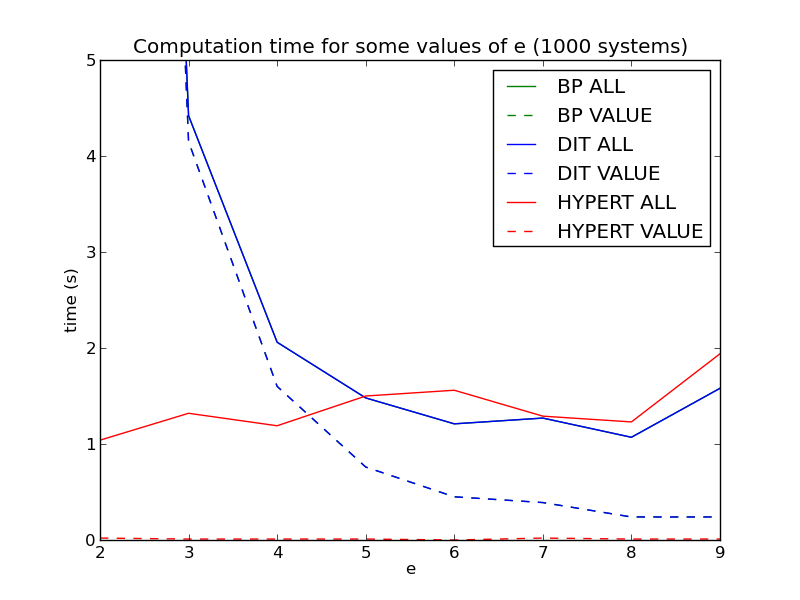
\includegraphics[width=0.9\textwidth]{../dit-simulation/plots/001_137389818886_princess.png}
    \end{center}
\end{frame}


\end{document}
